\documentclass[12pt, a4paper, oneside]{ctexart}
\usepackage{amsmath, amsthm, amssymb, bm, color, graphicx, geometry, mathrsfs,extarrows, braket, booktabs, array, xcolor, fontspec, appendix, float, subfigure, wrapfig, enumitem, titlesec}
\usepackage[colorlinks,linkcolor=red,anchorcolor=blue,citecolor=blue,urlcolor=blue,menucolor=black]{hyperref}

%%%% 设置中文字体 %%%%
% fc-list -f "%{family}\n" :lang=zh >d:zhfont.txt 命令查看已有字体
% \setCJKmainfont{方正新书宋_GBK.ttf}[BoldFont = 方正小标宋_GBK, ItalicFont = 方正楷体_GBK, BoldItalicFont = 方正粗楷简体]
\setCJKmainfont{方正新书宋_GBK.ttf}[BoldFont = 方正黑体_GBK.ttf, ItalicFont = simkai.ttf, BoldItalicFont = 方正粗楷简体.ttf]
%%%% 设置英文字体 %%%%
\setmainfont{Times New Roman}
\setsansfont{Calibri}
\setmonofont{Consolas}

%%%% 设置代码块 %%%%
% 在vscode中使用minted需要先配置python解释器, Ctrl+Shift+P, 输入Python: Select Interpreter选择安装了Pygments的Python版本. 再在setting.json中xelatex和pdflatex的参数中加入 "--shell-escape", 即可
% TeXworks中配置方法参考: https://blog.csdn.net/RobertChenGuangzhi/article/details/108140093
\usepackage{minted}
\renewcommand{\theFancyVerbLine}{
    \sffamily\textcolor[rgb]{0.5,0.5,0.5}{\scriptsize\arabic{FancyVerbLine}}} % 修改代码前序号大小
% 加入不同语言的代码块
\newmintinline{cpp}{fontsize=\small, linenos, breaklines, frame=lines}
\newminted{cpp}{fontsize=\small, baselinestretch=1, linenos, breaklines, frame=lines}
\newmintedfile{cpp}{fontsize=\small, baselinestretch=1, linenos, breaklines, frame=lines}
\newmintinline{matlab}{fontsize=\small, linenos, breaklines, frame=lines}
\newminted{matlab}{fontsize=\small, baselinestretch=1, mathescape, linenos, breaklines, frame=lines}
\newmintedfile{matlab}{fontsize=\small, baselinestretch=1, linenos, breaklines, frame=lines}
\newmintinline{python}{fontsize=\small, linenos, breaklines, frame=lines, python3}  % 使用\pythoninline{代码}
\newminted{python}{fontsize=\small, baselinestretch=1, linenos, breaklines, frame=lines, python3}  % 使用\begin{pythoncode}代码\end{pythoncode}
\newmintedfile{python}{fontsize=\small, baselinestretch=1, linenos, breaklines, frame=lines, python3}  % 使用\pythonfile{代码地址}

%%%% 设置行间距与页边距 %%%%
\linespread{1.2}
% \geometry{left=2.5cm, right=2.5cm, top=2.5cm, bottom=2.5cm}
\geometry{left=1.84cm,right=1.84cm,top=2.18cm,bottom=2.18cm}

%%%% 定理类环境的定义 %%%%
\newtheorem{example}{例}            % 整体编号
\newtheorem{theorem}{定理}[section] % 定理按section编号
\newtheorem{definition}{定义}
\newtheorem{axiom}{公理}
\newtheorem{property}{性质}
\newtheorem{proposition}{命题}
\newtheorem{lemma}{引理}
\newtheorem{corollary}{推论}
\newtheorem{condition}{条件}
\newtheorem{conclusion}{结论}
\newtheorem{assumption}{假设}
\numberwithin{equation}{section}  % 公式按section编号 (公式右端的小括号)
\newtheorem{algorithm}{算法}

%%%% 自定义环境 %%%%
\newsavebox{\nameinfo}
\newenvironment{myTitle}[1]{
    \begin{center}
    {\zihao{-2}\bf #1\\}
    \zihao{-4}\it
}{\end{center}}  % \begin{myTitle}{标题内容}作者信息\end{myTitle}
\newcounter{problem}  % 问题序号计数器
\newenvironment{problem}[1][]{\stepcounter{problem}\par\noindent\textbf{题目\arabic{problem}. #1}}{\smallskip\par}
\newenvironment{solution}[1][]{\par\noindent\textbf{#1解答. }}{\smallskip\par}  % 可带一个参数表示题号\begin{solution}{题号}
\newenvironment{note}{\par\noindent\textbf{注记. }}{\smallskip\par}
\newenvironment{remark}{\begin{enumerate}[label=\textbf{注\arabic*.}]}{\end{enumerate}}
\BeforeBeginEnvironment{minted}{\vspace{-0.5cm}}  % 缩小minted环境距上文间距
\AfterEndEnvironment{minted}{\vspace{-0.2cm}}  % 缩小minted环境距下文间距

%%%% 自定义段落开头序号,间距 (titlesec) %%%%
% 中文序号:\zhnum{section}, 阿拉伯序号:\arabic
\titleformat{\section}{\Large\bfseries}{\arabic{section}}{1em}{}[]
\titlespacing{\section}{0pt}{1.2ex plus .0ex minus .0ex}{.3ex plus .0ex}
\titlespacing{\subsection}{0pt}{1.2ex plus .0ex minus .0ex}{.3ex plus .0ex}
\titlespacing{\subsubsection}{0pt}{1.2ex plus .0ex minus .0ex}{.3ex plus .0ex}

%%%% 图片相对路径 %%%%
\graphicspath{{figures/}} % 当前目录下的figures文件夹, {../figures/}则是父目录的figures文件夹
\setlength{\abovecaptionskip}{-0.2cm}  % 缩紧图片标题与图片之间的距离
\setlength{\belowcaptionskip}{0pt} 

%%%% 缩小item,enumerate,description两行间间距 %%%%
\setenumerate[1]{itemsep=0pt,partopsep=0pt,parsep=\parskip,topsep=5pt}
\setitemize[1]{itemsep=0pt,partopsep=0pt,parsep=\parskip,topsep=5pt}
\setdescription{itemsep=0pt,partopsep=0pt,parsep=\parskip,topsep=5pt}

%%%% 自定义公式 %%%%
\everymath{\displaystyle} % 默认全部行间公式, 想要变回行内公式使用\textstyle
\DeclareMathOperator*\uplim{\overline{lim}}     % 定义上极限 \uplim_{}
\DeclareMathOperator*\lowlim{\underline{lim}}   % 定义下极限 \lowlim_{}
\DeclareMathOperator*{\argmax}{arg\,max}  % 定义取最大值的参数 \argmax_{}
\DeclareMathOperator*{\argmin}{arg\,min}  % 定义取最小值的参数 \argmin_{}
\let\leq=\leqslant % 简写小于等于\leq (将全部leq变为leqslant)
\let\geq=\geqslant % 简写大于等于\geq (将全部geq变为geqslant)
\DeclareRobustCommand{\rchi}{{\mathpalette\irchi\relax}}
\newcommand{\irchi}[2]{\raisebox{\depth}{$#1\chi$}} % 使用\rchi将\chi居中

%%%% 一些宏定义 %%%%
\def\bd{\boldsymbol}        % 加粗(向量) boldsymbol
\def\disp{\displaystyle}    % 使用行间公式 displaystyle(默认)
\def\tsty{\textstyle}       % 使用行内公式 textstyle
\def\sign{\text{sign}}      % sign function
\def\wtd{\widetilde}        % 宽波浪线 widetilde
\def\R{\mathbb{R}}          % Real number
\def\N{\mathbb{N}}          % Natural number
\def\Z{\mathbb{Z}}          % Integer number
\def\Q{\mathbb{Q}}          % Rational number
\def\C{\mathbb{C}}          % Complex number
\def\K{\mathbb{K}}          % Number Field
\def\P{\mathbb{P}}          % Polynomial
\def\d{\mathrm{d}}          % differential operator
\def\e{\mathrm{e}}          % Euler's number
\def\i{\mathrm{i}}          % imaginary number
\def\re{\mathrm{Re}}        % Real part
\def\im{\mathrm{Im}}        % Imaginary part
\def\res{\mathrm{Res}}      % Residue
\def\ker{\mathrm{Ker}}      % Kernel
\def\vspan{\mathrm{vspan}}  % Span  \span与latex内核代码冲突改为\vspan
\def\L{\mathcal{L}}         % Loss function
\def\O{\mathcal{O}}         % big O notation
\def\wdh{\widehat}          % 宽帽子 widehat
\def\ol{\overline}          % 上横线 overline
\def\ul{\underline}         % 下横线 underline
\def\add{\vspace{1ex}}      % 增加行间距
\def\del{\vspace{-1.5ex}}   % 减少行间距

%%%% 正文开始 %%%%
\begin{document}

%%%% 以下部分是正文 %%%%  
\clearpage
\begin{myTitle}{NLP期末复习}
    强基数学002\quad 吴天阳
\end{myTitle}
\section{文本预处理}
\begin{definition}[形符化]
    将文本分解为词、短语、符号式等其他有意义的形符(token)元素的过程.
\end{definition}
\begin{remark}
    \item 形符化可发生在不同程度的颗粒度:一个文本可分解为段落、句子、音节、音素.
    \item 形符序列可作为其他进一步处理的输入.(如句法分析,文本分类等)
    \item 形符化可用于:信息检索,信息抽取,拼写检查.
\end{remark}

\paragraph{一、文本预处理的三个基本任务}
\begin{itemize}
    \item 行文中的词切分及词的形符化.
    \item 词形的归一化.
    \item 行文中的句子划分.
\end{itemize}

\paragraph{二、什么是词?}以下两个定义常用于英文语法中:

\textbf{词元(Lemma)}:具有相同词干,主要词性及相似词义的词汇集合.(词典用于存储词元)

\textbf{词形(Wordform)}:词在形式上的曲折变化.(构成词语的规模)\\
例:cat与cats有相同的词元,不同的词形.

\paragraph{三、汉语分词中切分歧义}
\begin{enumerate}
    \item 交集型切分歧义:汉字串为ABC,其中AB与AC同时成词,则称为交集型切分歧义.
    \item 组合型切分歧义:汉字串为AB,其中A、B、AB同时成词,则称之为组合型切分歧义.
    \item 混合型切分歧义:既是交集型切分歧义又是组合型切分歧义.
\end{enumerate}
\noindent 例:“网球/场、网/球场”为交集型,“他站/起/身/来、他站/起身/来”为组合型,
“这样的/人/才能/成大器、这样的/人才/能/成大器、这样的/人才能/成大器”为混合型.

简单的切分算法:最大匹配.(正向最大匹配、反向最大匹配、双向最大匹配) 更好的算法:概率模型(隐马尔可夫模型)

\paragraph{四、归一化}包括词元、词干及大小写的归一化.
\begin{itemize}
    \item \textbf{词元化}:将词的曲折变化转化为词的基本型(这一操作将文本中的词映射到词典中的词)\\
    例:am,is,are→be;\ car, cars, car's, cars' → car;\\
    the boy's cars are different colors → the boy car be different color.
    \item \textbf{词干化}:将次的曲折变化转化为词根.\\
    例:catlike, catty → cat;\ stemmer, stemming, stemmed → stem.
    \item \textbf{大小写归一化}:将所用字母的大小写全部转化为小写,句子中的大写除外.\\
    \textit{因为对机器翻译、情感分析等任务来说,大小写很重要.}
\end{itemize}
\paragraph{五、最小编辑距离}
\begin{definition}
最小编辑距离(minimum edit distance)指两个字符串之间进行如下编辑操作的最小
次数:
\begin{itemize}
    \item Insertion(插入)
    \item Delection(删除)
    \item Substitution(替换)
\end{itemize}
\end{definition}
\begin{solution}
设两个长度为$n,m$字符串分别为$a = \{a_1,\cdots, a_n\},\ b=\{b_1,\cdots,b_m\}$,函数$f(i,j),\ (i\in[1,n],j\in[1,m])$表示
字符串$a$中前$i$个字符转化为字符串$b$中前$j$个字符的最小编辑距离,则$f(n,m)$表示将字符串$a$转化为字符串$b$所用的最小编辑距离,
且$f(i,j)$满足一下递推式:
\begin{align*}
    f(i,j) =&\ \begin{cases}
        f(i-1,j-1),&\quad a_i = b_j,\\
        \min\{f(i-1,j-1),f(i-1,j),f(i,j-1)\},&\quad a_i\neq b_j.
    \end{cases}\\
    \text{初始化 } f(i, j) =&\ \begin{cases}
        i,&\quad j = 0,\\
        j,&\quad i = 0,\\
        +\infty,&\quad \text{否则}.
    \end{cases}
\end{align*}
上述递推式的含义:
\begin{itemize}
    \item 若$a_i=b_j$,则说明当前字符串末端字符相同,于是最小编辑距离直接从$f(i-1,j-1)$转移得到;
    \item 若$a_i\neq b_j$,则说明当前字符串末端字符不相同,需要从上述三种修改方式中选择一种:
    \begin{enumerate}
        \item “替换” $f(i-1,j-1)+1$:将$a_i$直接替换为$b_j$,再从$f(i-1,j-1)$转移.
        \item “删除” $f(i-1, j)+1$:将$a_i$删除,再从$f(i-1,j)$转移.
        \item “插入” $f(i,j-1)+1$:将$a_i$后插入字符$b_j$,再从$f(i,j-1)$转移.
    \end{enumerate}
\end{itemize}
通过回退指针记录每次最小编辑距离从哪转移过来的,计算完全部状态之后,从$f(n,m)$开始回退,从而得到两个字符串的具体编辑操作.
算法的时间复杂度为$\O(nm)$.
\end{solution}
\section{概率语言模型}
\subsection{概念}
概率语言模型解决的问题:对于给定词串$w = \{w_1,\cdots, w_n\}$,计算词串$w$是通顺句子的概率$p(w)$.\\
广义上讲,用于计算$p(w)$或$p(w_n|w_1,\cdots, w_{n-1})$的模型均为语言模型(language model).

由条件概率定义可知:$p(w_1,\cdots, w_n) = p(w_1)p(w_2|w_1)p(w_3|w_1,w_2)\cdots p(w_n|w_1,\cdots, w_{n-1})$,
假设给定语料库$C$(大量语言使用数据),通过极大似然估计(MLE)可以得到:
\begin{equation*}
    p(w_m|w_1,\cdots,w_{m-1}) = \frac{c(w_1,\cdots, w_{m-1},w_m)}{c(w_1,\cdots, w_{m-1})}
\end{equation*}
其中$c(w_1,\cdots, w_{m-1}) = \sum_{w_j\in W}c(w_1,\cdots, w_{m-1}, w_j)$表示文本串$\{w_1,\cdots, w_{m-1}\}$
作为子串在语料库$C$中的出现次数.

该方法是基于\textbf{当前词出现的概率依赖于它前面的词},缺点是当$m$非常大时,$c(w_1,\cdots, w_m)$可能为$0$,
导致条件概率无法计算. 考虑到一个词可能仅与前面相对位置较近的词相关,距离越远的词相关越差,只考虑相对位置较近的词出现概率,
于是就有了下面的n-gram模型.
\subsection{n-gram模型}
\begin{definition}[Markov假设]
    位于某个特定状态的概率,取决于前$n-1$个状态,即
    \begin{equation*}
        P(w_i|w_1,\cdots, w_{i-1})\approx P(w_i | w_{i-n+1},\cdots,w_{i-1})
    \end{equation*}
    则称$w = \{w_1,\cdots, w_m\}$为一个$n-1$阶Markov链.
\end{definition}
应用于语言模型中,就是指句子中每个词出现的概率仅取决于它前$n-1$个词,称为\textbf{$N$元语言模型(n-gram模型)},也称为
狭义语言模型. 下面举几个例子:
\begin{itemize}
    \item \textbf{1-gram模型(unigram)}:$p(w_1,\cdots, w_n)\approx p(w_1)p(w_2)\cdots p(w_n)$;
    \item \textbf{2-gram模型(bigram)}:$p(w_1,\cdots, w_n)\approx p(w_1)p(w_2|w_1)p(w_3|w_2)\cdots p(w_n|w_{n-1})$;
    \item \textbf{3-gram模型(trigram)}:$p(w_1,\cdots, w_n)\approx p(w_1)p(w_2|w_1)p(w_3|w_1,w_2)\cdots p(w_n|w_{n-2},w_{n-1})$.
\end{itemize}
\noindent 以“please close the door”为例:(均加入了起始符START和结束符END)\\
2-gram模型为p(please,close,the,door)=p(please|START)p(close|please)$\cdots$p(door|the)p(END|door);\\
3-gram模型为p(please,close,the,door)=p(please|START)p(close|START,please)$\cdots$p(END|the,door).

\begin{example}[拼音转化句子问题]
    给定拼音串$a$,求出最有可能对应的句子.
\end{example}
\begin{solution}
设$C$表示拼音串$a$全部可能对应的句子集合,则最有可能对应的句子$c$应该满足
    \begin{align*}
        c =&\ \argmax_{c\in C}p(c|a) = \argmax_{c\in C}\frac{p(a|c)p(c)}{p(a)} = \argmax_{c\in C}p(c)
    \end{align*}
    我们假设在每个句子在$C$中的出现次数均等,则$p(c|a)$为常数,于是问题转化为求出$C$中哪个句子最有可能是完整的句子.
    于是使用n-gram模型求出每个句子$c$的$p(c)$,取最大的$p(c)$对应的句子即可.
\end{solution}
\textbf{注}:n-gram中的N不宜太大,在n-gram中参数个数为$|W|^N$,$|W|$表示词库的大小,一般来说3-gram最为常用,
n-gram是一个基于样本的模型. 由于n-gram模型非常依赖于语料库C,若某个词组在C中没有出现,则无法计算条件概率,所以需要对其进行处理.

\subsection{数据稀疏}
\begin{definition}[Zipf定律]
    在自然语言的语料库中,一个单词出现的频率与它在频率表中的排名称反比.
\end{definition}
缓解数据稀疏的方法:
\begin{enumerate}
    \item \textbf{平滑}:重新估计零概率及低值概率,赋予它们一个非零值.
    \item \textbf{回退}:高阶n-gram的概率难以计算时,用较低阶的进行估计.
\end{enumerate}
\subsubsection{Laplace平滑(加一平滑)}
设词库大小为$|V|$,$N$为语料库中词形的总数,\add $c_i=c(w_i)$为词$w_i$在语料库中出现次数, 
则unigram中MLE值为$p(w_i) = \frac{c_i}{N}$,
在加一平滑中MLE值为$p_{Laplace}(w_i) = \frac{c_i+1}{N+|V|}$,\add 记$c^*_i = \frac{(c_i+1)N}{N+|V|}$
为$c_i$的\textbf{加一折扣计数}.

对于n-gram问题中,$w_i$的加一平滑的MLE值为
\begin{equation*}
    p(w_i|w_{i-n+1},\cdots, w_{i-1}) = \frac{c(w_{i-n+1},\cdots, w_i)+1}{c(w_{i-n+1},\cdots,w_{i-1})+|V|}   
\end{equation*}
加一折扣计数为
\begin{equation*}
    c^*_i(w_{i-n+1},\cdots,w_i) = \frac{(c(w_{i-n+1},\cdots,w_i)+1)c(w_{i-n+1},\cdots,w_{i-1})}{c(w_{i-n+1},\cdots,w_{i-1})+|V|}
\end{equation*}
通过L3 Language Model.ppt中第40页例子可以较好的掌握加一平滑的原理,考试中有可能出此类题目. 在加一平滑的基础上,将$1$改为$\delta$,其中$\delta\in [0,1]$,
称为Lidstone平滑(加Delta平滑),其MLE如下
\begin{equation*}
    p(w_i|w_{i-n+1},\cdots, w_{i-1}) = \frac{c(w_{i-n+1},\cdots, w_i)+\delta}{c(w_{i-n+1},\cdots,w_{i-1})+|V|\delta},\quad \delta\in[0,1].
\end{equation*}
可通过在验证集上的交叉验证确定$\delta$的值.\textit{(Good-Turing平滑感觉不会考,没有例题)}

\subsubsection{回退法}
回退法就是在条件概率无法计算时,通过逐步减小$n$的大小直到找到可以计算的条件概率,用其代替无法计算的值,以3-gram(trigram)的回退法为例
\begin{equation*}
    p(w_{i}|w_{i-2},w_{i-1}) = \begin{cases}
        p(w_i|w_{i-2},w_{i-1}),&\quad c(w_{i-2},w_{i-1},w_{i}) > 0,\\
        \alpha_1 p(w_i|w_{i-1}),&\quad c(w_{i-2},w_{i-1},w_i) = 0\text{且}c(w_{i-1},w_i) > 0,\\
        \alpha_2 p(w_i),&\quad \text{否则}.
    \end{cases}
\end{equation*}
\subsubsection{插值法}
插值法与回退法类似,当遇到无法计算的条件概率时,将其令为$0$,还是以3-gram(trigram)为例:
\begin{equation*}
    p(w_i|w_{i-2},w_{i-1}) = \lambda_1p(w_n)+\lambda_2p(w_n|w_{n-1})+\lambda_3p(w_n|w_{n-2},w_{n-1})
\end{equation*}
其中$\lambda_i\in[0,1],\ \sum_{i=1}^3\lambda_i = 1$.
\subsection{模型评估}
在测试集上评估两个语言模型,由困惑度和信息熵作为估计标准.
\begin{definition}[困惑度,Perplexity]
    设测试集语句$W=\{w_1,\cdots,w_n\}$上使用bigram模型,则困惑度的定义为$p(w_2|w_1),\cdots,p(w_n|w_{n-1})$的几何平均数倒数:
    \begin{equation*}
        PP(W) = p(W)^{-\frac{1}{n}} = \left[\prod_{i=1}^np(w_i|w_{i-1})\right]^{-\frac{1}{n}}
    \end{equation*}
\end{definition}
\textbf{注}:困惑度可以理解为,如果$W$是正确句子,则$p(W)$应该都拥有较高概率值,则困惑度应该较小.

\begin{definition}[信息熵]
    语句$W = \{w_1,\cdots, w_n\}$的信息熵和平均信息熵定义如下,其中$q(W)$表示语句$W$是正确语句的概率:
    \begin{align*}
        \text{信息熵:} H(W) =&\ -\sum_{i=1}^nq(w_1,\cdots, w_i)\log_2q(w_1,\cdots, w_i)\\
        \text{平均信息熵:} H(W) =&\ -\frac{1}{n}\sum_{i=1}^nq(w_1,\cdots, w_i)\log_2q(w_1,\cdots, w_i)
    \end{align*}
    语言$L$的信息熵为
    \begin{align*}
        H(L) =&\ -\lim_{n\to\infty}\frac{1}{n}\sum_{i=1}^nq(w_1,\cdots,w_i)\log_2q(w_1,\cdots,w_i)\\
        =&\ -\lim_{n\to\infty}\frac{1}{n}\log_2q(w_1,\cdots,w_n)
    \end{align*}
\end{definition}
由于$q(\cdot)$未知,在n-gram中,使用$p(\cdot)$作为$q(\cdot)$的估计,若$N$充分大,则有
\begin{equation*}
    H(W) = -\frac{1}{n}\log_2p(w_1,\cdots,w_n)
\end{equation*}
于是$PP(W) = 2^{H(W)}$,也就是说明$H(W)$越小,则$PP(W)$越小,模型性能越好.
\subsection{语言模型的应用}
\paragraph{基于语言模型的分词方法}
对于待切分的句子$S = {w_1,\cdots,w_n}$,取长度为$1\leq k\leq n$的前缀$W = {w_1,\cdots,w_k}$,
一个最简单的做法确定$W$中的最优分词:
\begin{align*}
    \widehat{W} = \argmax_{W}p(W|S) = \argmax_{W}p(W)p(S|W) \approx \argmax_{W}p(W)
\end{align*}
但这样假设了$p(S|W)$为常数,也就是将词组$W$视为独立的统计单元,效果不好. 可通过对句子中的词进行词性标注,然后对不同标注设定不同的生成模型
$p(S|C)$. \textit{该过程较为复杂,应该不考.}
\subsection{信息论知识}
\begin{definition}[熵]
    设$X\sim p(x)$是离散随机变量,$p(x)$为$X$服从的概率质量函数,则$X$的熵为
    \begin{equation*}
    H(X) = -\sum_{x\in X}p(x)\log_2p(x)   
    \end{equation*}
    约定$0\log 0 = 0$. 有时将$H(X)$记为$H(p)$.
\end{definition}
熵用于描述一个随机变量的不确定性的数量,单位为二进制位比特(bit).
\begin{definition}[联合熵]
    设$X,Y\sim p(x,y)$是服从$p(x,y)$的一对离散型随机变量,则$X,Y$的联合熵为
    \begin{equation*}
        H(X,Y) = -\sum_{x\in X}\sum_{y\in Y}p(x,y)\log_2 p(x,y)
    \end{equation*}
\end{definition}
\begin{definition}[条件熵]
    设$X,Y\sim p(x,y)$是服从$p(x,y)$的一对离散型随机变量,则$X,Y$的条件熵为
    \begin{equation*}
        H(X|Y) = \sum_{x\in X}\sum_{y\in Y}p(x,y)\log_2 p(y|x)
    \end{equation*}
\end{definition}
\textbf{性质}:$H(X,Y) = H(X)+H(Y|X)$
\section{文本分类}
使用机器学习对文本进行分类,需要以下几步:
\begin{enumerate}
    \item 预处理(除去停用词,提取词干)
    \item 文本表示(向量空间模型)
    \item 分类模型
    \item 评价
\end{enumerate}
\noindent\textbf{停用词}:高频词往往携带较少信息,将停用词删去.\\
\textbf{词干}:词的后缀进行变形处理,将相同概念意义的词进行合并.\\
\textbf{向量空间(词袋)模型}:将文本表示为由词条构成的向量. 使用该模型需要假设词之间相互独立,即不考虑词在文本中出现的顺序,将文本视为词集合,
也称文本为\textbf{词袋(bag-of-words)}.

\subsection{词的权重}
设总共包含$N$个文档,经过预处理后文档中包含的词条总数为$M$,第$k$个词条在第$i$个文档中出现的次数记为$f_{ik}$,第$k$个词条在文档集合中出现的总次数记为$n_k$.

\textbf{文档-词条矩阵}$A = (a)_{ik}$,第$i$行表示第$i$篇文档由词构成的向量,$a_{ik}$表示第$i$个文档中第$k$个词条的权重,
\begin{equation*}
    A = \left[\begin{matrix}
        a_{11}&a_{12}&\cdots&a_{1M}\\
        a_{21}&a_{22}&\cdots&a_{2M}\\
        \vdots&\vdots&\ddots&\vdots\\
        a_{N1}&a_{N2}&\cdots&a_{NM}
    \end{matrix}\right]
\end{equation*}
主要有以下四种权重:
\begin{itemize}
    \item \textbf{布尔权重}:若词在文档中出现则为$1$,否则为$0$,$a_{ik} = \begin{cases}
        1,&f_{ik} > 0,\\
        0,&\text{否则}.
    \end{cases}$
    \item \textbf{词条频次(term frequency, tf)}:词条在文档中出现频次作为权重,$a_{ik} = f_{ik}$.
    \item \textbf{逆文档频次(inverse document frequency, idf)}:词条的权重与在文档集合中出现次数成反比,$a_{ik}\propto \frac{1}{n_k}$.
    \item \textbf{tf$\times$idf权重}:同时考虑词条频次和逆文档频次,$a_{ik} = f_{ik}\log\left(N/n_k\right)$.
\end{itemize}
\subsection{分类模型}
\subsubsection{k-近邻}
基于训练集$D=\{(\bd{x_i},y_i):1\leq i\leq n\}$,对于每个样例$(\bd{x},y)$,在$D$中找出最靠近$\bd{x}$的$k$个样本$\bd{x}_{i_1},\bd{x}_{i_2},\cdots,\bd{x}_{i_k}$,
返回这$k$个样本中出现次数最多的标签值作为预测结果.

可采用交叉验证寻找最优的$k$值,距离的选择有欧氏距离(L2范数),余弦距离$\cos\theta = \frac{(\bd{x},\bd{x_i})}{||\bd{x}||_2||\bd{x}_i||_2}$.

优点:可描述复杂的分类边界,训练快速,简单好用,模型解释性好;

缺点:存储开销大,样本不均匀影响,参数空间较大导致搜索速度降低,效率不高.

\subsubsection{朴素贝叶斯}
朴素贝叶斯是基于贝叶斯公式,通过先验知识预测类别.

贝叶斯公式为$p(c_k|x) = \frac{p(x|c_k)p(c_k)}{p(x)}$,\add 表示文档$x$预测为$c_k$的概率,
其中文档权重向量$x = (x_1,\cdots,x_M)^T$,
其中$x_i$表示$i$个词条在文档$x$中的出现频率,朴素贝叶斯的假设是$X_1,\cdots,X_M$
是\textbf{相互独立}的,于是$p(X|c_k) = p(X_1,\cdots,X_M|c_k) = p(X_1|c_k)p(X_2|c_k)\cdots p(X_M|c_k)$.

朴素贝叶斯的预测方法就是使用贝叶斯公式,\add 只不过由于直接计算概率值可能出现精度溢出,所以推导过程中取了$log$,
通过$p(x|c_k) = \frac{p(x,c_k)}{p(c_k)}$\add 可以求出在训练集中$x$在类别$c_k$的文档中出现的概率,由于是离散取值,
所以可以假设为多项分布,$p(X_i|c_k)$的含义是第$i$个词条在类别为训练集中类别为$c_i$文档中的出现次数.

设总共有$d$个类别,
则文档$x$的预测类别为:
\begin{align*}
    \hat{c} =&\ \argmax_{1\leq k\leq d}p(c_k|x) = \argmax_{1\leq k\leq d}\frac{p(c_k)p(x|c_k)}{p(x)} = \argmax_{1\leq k\leq d}p(c_k)p(x|c_k)\\
    =&\ \argmax_{1\leq k\leq d}\log p(c_k) + \log p(x|c_k) = \argmax_{1\leq k\leq d}\log p(c_k) + \log\prod_{i=1}^Mp(X_i|c_k)^{x_i}\\
    =&\ \argmax_{1\leq k\leq d}\underbrace{\log p(c_k)}_{w_0^{(k)}} + \sum_{i=1}^Mx_i\underbrace{\log p(X_i|c_k)}_{w_i^{(k)}}
\end{align*}
记$\bd{w}^{(k)} = (w_0^{(k)}, w_1^{(k)},\cdots, w_M^{(k)})^T$,$\bd{x}'=(1,x_1,\cdots,x_n)^T$,则上式预测还可简写为
\begin{equation*}
    \hat{c} = \argmax_{1\leq k\leq d}\bd{x}^T\bd{w}^{(k)}
\end{equation*}
\subsection{模型评价}
实验设置(3种):
\begin{itemize}
    \item 将数据集划分为训练集和测试集;
    \item \textbf{$n$倍交叉验证},将数据集划分为$n$份,每次取其中$n-1$份作为训练集,其中剩余的一份作为测试集,独立地做$n$次,以$5$轮测试的平均性能作为模型的性能.
    \item \textbf{保留测试},将数据集划分为训练集、验证集和测试集,训练集中学习模型参数,验证集中调整超参数,测试集中对模型进行评估.
\end{itemize}
若是二分类问题,可用\textbf{混淆矩阵(困惑矩阵)}对模型性能进行评价,混淆矩阵的行表示样本标签(真实值),列表示预测结果(预测值),如下图所示
\begin{figure}[htbp]
    \centering
    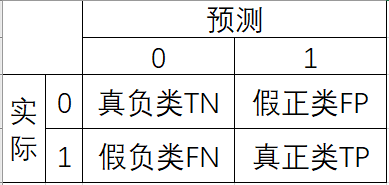
\includegraphics[scale=1.6]{混淆矩阵.png}
\end{figure}

两个常用参数为\textbf{精度(Precision)}:$P = \frac{TP}{TP+FP}$,\textbf{召回率(Recall)}:$R = \frac{TP}{TP+FN}$,一种评估精度与召回率的参数为
$F_1$参数(两者的调和平均数):$F_1 = \frac{2}{\frac{1}{P}+\frac{1}{R}}$. 一般来说$F_1$参数越大模型效果越好.
\end{document}
